\section{Tranzitivnost in goste orbite}

\begin{izrek}[Topološka tranzitivnost] \label{thm:transitivity}
    Če sta \(U, V \subseteq \CC\) odprti, potem obstaja tak \(n \geq 0\), da velja \(f^{n} (U) \cap V \neq \emptyset\).
\end{izrek}

\noindent Pomagamo si z naslednjimi pomožnimi rezultati.

\begin{trditev}[Širjenje vzdolž ubežnih orbit]
    Naj bo \(z_0 \in I (f)\) in \(z_n = f^n (z_0)\) za \(n \in \NN\). Potem je \(\lim_{n \to \infty} \re z_n = \infty\).
\end{trditev}

\begin{dokaz}
    Ker za vsak \(n \geq 0\) velja \(z_{n + 1} = e^{z_n}\). Zato je po definiciji \(I (f)\)
    \[\lim_{n \to \infty} \re z_n = \lim_{n \to \infty} \log |z_{n + 1}| = \infty.\]
    Poleg tega je \(\lim_{n \to \infty} |f' (z_n)| = \lim_{n \to \infty} |f (z_n)| = \lim_{n \to \infty} |z_{n + 1}| = \infty\). Zato obstaja \(N \in \NN\), da za vsak \(n \geq N\) velja \(|f' (z_n)| \geq 2\). Za \(m > N\) izračunamo odvod \(f^{m} = f^{m - N} \circ f^{N}\) po verižnem pravilu:
    \[|(f^{m})' (z_0)| = \abs{ \prt{f^{N}}' (z_0) } \cdot \prod_{n = N}^{m - 1} |f' (z_n)| \geq 2^{m - N} \cdot \abs{ \prt{f^{N}}' (z_0) }.\]
    Za vsak \(z \in \CC\) velja \(f' (z) \neq 0\) in zato \(|(f^N)' (z_0)| \neq 0\). Zato sklepamo
    \[\lim_{m \to \infty} |(f^{m})' (z_0)| = \infty.\]
\end{dokaz}

\begin{trditev}[Mali diski eksplodirajo] \label{prop:small_disks}
    Naj bo \(z_0 \in I (f)\) in \(z_n = f^{n} (z_0)\). Opazujemo diske \(D_n \coloneq D_{2 \pi} (z_n)\). Potem obstaja \(n_0 \in \NN\) in zaporedje \(\left\{ \phi_n \right\}_{n = n_0}^{\infty}\) holomorfnih preslikav \(\phi_n \colon D_n \to \CC\) z naslednjimi lastnostmi:
    \begin{enumerate}
        \item \label{item:ena} \(\phi_n (z_n) = z_0\);
        \item \label{item:dva} za vsak \(z \in D_n\) velja \(f^n (\phi_n (z)) = z\);
        \item \label{item:tri} \(\lim_{n \to \infty} \sup_{z \in D_n} |\phi_n' (z)| = 0\);
        \item \label{item:stiri} \(\lim_{n \to \infty} \diam (\phi (D_n)) = 0\).
    \end{enumerate}
\end{trditev}

\begin{dokaz}
    Naj bo \(z \in D_n\). Potem po Lagrangeevem izreku velja
    \begin{equation}
        |\phi_n (z) - \phi_n (z_n)| \leq |z - z_0| \cdot \sup_{\zeta \in D_n} |\phi_n' (\zeta)| \leq 2 \pi \sup_{\zeta \in D_n} |\phi_n' (\zeta)|.
    \end{equation}
    Predpostavimo točko \ref{item:tri} in vidimo
    \[\lim_{n \to \infty} \diam \prt{\phi \prt{D_n}} \leq \lim_{n \to \infty} 4 \pi \sup_{\zeta \in D_n} \abs{\phi_n' (\zeta)} = 0.\]
    Torej točka \ref{item:tri} implicira točko \ref{item:stiri}.

    Za začetek privzamemo, da za vsak \(n \in \NN\) velja \(\absolute{z_n} \geq 2 \pi + 2\). Tako noben disk \(D_n\) ne vsebuje izhodišča. Za vsak \(n \in \NN\) naj bo \(L_n \colon D_n \to \CC\) veja logaritma, tako da je \(L_n (z_n) = L_n (e^{z_{n - 1}}) = z_{n - 1}\). Po predpostavki za vsak \(z \in D_n\) velja \(\absolute{z} \geq 2\) in zato
    \[\absolute{L_n' (z)} = \frac{1}{\absolute{z}} \leq \frac{1}{2}.\]
    Spet upoštevamo Lagrangeev izrek in vidimo, da za vsak \(n\) in vsak \(z \in D_n\) velja
    \[\absolute{L_n (z) - z_{n - 1}} = \absolute{L_n (z) - L_n (z_n)} \leq 2 \pi \cdot \sup_{\zeta \in D_n} \absolute{L_n' (\zeta)} \leq \pi.\]
    Z indukcijo sklepamo, da je kompozitum \(\phi_n \coloneq L_1 \circ L_2 \circ \dots \circ L_n\) definiran na \(D_n\) in za vsak \(z \in D_n\) velja \(\absolute{\phi_n' (z)} \leq 2^{-n}\). Torej za preslikavo \(\phi_n\) velja točka \ref{item:tri}, točki \ref{item:ena} in \ref{item:dva} pa veljata po konstrukciji.

    Če predpostavka \(\absolute{z_n} \geq 2 \pi + 2\) ne velja, sklepamo takole. Ker je \(z_0\) ubežna točka, še vedno obstaja tak \(n_1 \in \NN\), da za vsak \(n > n_1\) velja \(\absolute{z_n} \geq 2 \pi + 2\). To pa pomeni, da za vsak tak \(n\) obstaja holomorfna preslikava \(\psi_n \colon D_n \to D_{n_1}\), za katero veljajo vse točke trditve, tako, da za \(z_0\) izberemo \(z_{n_1}\). Po izreko o inverzni funkciji zdaj obstaja okolica \(U\) točke \(z_{n_1}\) in veja \(\pi \colon U \to \CC\) preslikave \(f^{- n_1}\), ki \(z_{n_1}\) preslika v \(z_0\).

    Naj bo \(K\) majhen zaprt disk okrog \(z_{n_1}\), tako da je \(K \subset U\). Po točki \ref{item:stiri} za dovolj velik \(n\) velja \(\psi_n (D_n) \subset K\). Tako lahko definirmo
    \[\phi_n \colon D_n \to \CC; \qquad \phi_n (z) \coloneq \pi (\psi (z)).\]
    Taka preslikava po definiciji zadošča točki \ref{item:ena} in \ref{item:dva} in po točki \ref{item:tri}, ki velja za \(\psi_n\), velja
    \[\sup_{z \in D_n} \absolute{\phi_n' (z)} = \sup_{z \in D_n} \prt{\absolute{\psi_n' (z)} \cdot \absolute{\pi' (\psi_n (z))}} \leq \max_{z \in D_n} \absolute{\psi_n' (z)} \cdot \sup_{w \in K} \absolute{\pi' (w)}.\]
    Ker je \(K\) kompaktna, zvezna funkcija \(\absolute{pi'}\) na njej zavzame svoj maksimum, ki je neodvisen of \(n\). Zato je
    \[\lim_{n \to \infty} \max_{z \in D_n} \absolute{\psi_n' (z)} \cdot \sup_{w \in K} \absolute{\pi' (w)} = 0 \qquad\]
    in posledično
    \[\lim_{n \to \infty} \sup_{z \in D_n} \absolute{\phi_n' (z)} = 0.\]
\end{dokaz}

\begin{trditev}[Slike velikih diskov] \label{prop:lare_disks}
    Naj bo \(K\) neprazna kompaktna podmnožica \(\CC \setminus \set{0}\). Potem obstaja \(\rho > 0\) tako da velja naslednje. Naj bo \(D\) disk z radijem \(2 \pi\) s središčem v točki \(\zeta\), za katero velja \(\re (\zeta) \geq \rho\). Potem je \(K \subset f^2 (D)\).
\end{trditev}

\begin{dokaz}
    Disk \(D\) vsebuje zaprt kvadrat \(S\) s stranico dolžine \(2 \pi\), prav tako s središčem v \(\zeta\). Naj bo \(a = \re (\zeta) - \pi\) realni del leve navpične stranice \(S\). Potem je \(a + 2 \pi = \re (\zeta) + \pi\) realni del desne navpične stranice \(S\). Preslikava \(f\) kvadrat \(S\) preslika v krožni kolobar \(A\) s središčem v izhodišču, notranjim radijem \(r_{-} = e^a\) in zunanjim radijem \(r_{+} e^{a + 2 \pi}\) (glej sliko \ref{fig:exponential}).
    \begin{figure}
        \centering
        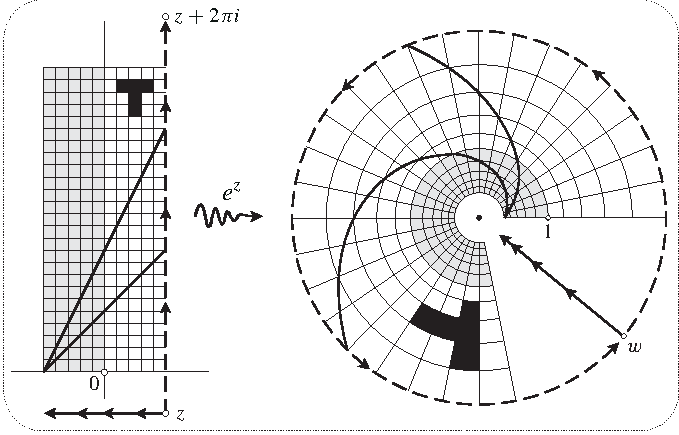
\includegraphics[width=0.6\textwidth]{needham_figure.pdf}
        \caption[Geometrijsko delovanje kompleksne eksponentne preslikave]{Geometrijska vizualizacija kompleksne eksponentne preslikave. Ilustracija iz knjige \cite{Needham_1997}}
        \label{fig:exponential}
    \end{figure}
    Če je \(a\) dovolj velik, je kolobar \(A\) dovolj širok, da vsebuje pravokotnik višine \(2 \pi\). Slika tega pravokotnika nato pokrije večino kompleksne ravnine, vključno s kompaktno množico \(K\). Bolj natančno; naj bo \(a \geq 0\) in zato \(r_+ - r_- \geq e^{2 \pi} > 2 \pi\). Torej \(A\) vsebuje pravokotnik \(R\) višine \(2 \pi\), tako kot je prikazano na sliki \ref{fig:transitivity}.
    \begin{figure}%
        \centering
        \begin{tikzpicture}
\tikzset{desnozgoraj/.style={anchor=base west, yshift=3pt, xshift=-2pt}}
\tikzset{levozgoraj/.style={anchor=base east, yshift=3pt, xshift=2pt}}
\tikzset{desnospodaj/.style={anchor=base west, yshift=-12pt, xshift=-2pt}}
\tikzset{levospodaj/.style={anchor=base east, yshift=-12pt, xshift=2pt}}
\tikzset{sredinaspodaj/.style={anchor=base, yshift=-12pt}}
\definecolor{siva}{gray}{0.8} 

\begin{scope}[shift={(0,0)}]
    \draw[->] (-0.5,0) -- (3.5,0);
    \draw[->] (0,-2.5) -- (0,2.5);

    \pgfmathsetmacro{\r}{1.1}
    \pgfmathsetmacro{\xo}{2}
    \pgfmathsetmacro{\yo}{1.3}
    \pgfmathsetmacro{\xl}{{2-\r/2}}
    \pgfmathsetmacro{\xr}{{2+\r/2}}

    \draw[dashed] (\xl, 0) -- (\xl, {\yo-\r/2});
    \draw[dashed] (\xr, 0) -- (\xr, {\yo-\r/2});

    \draw (\xo, \yo) circle ({\r})
        node[above left, xshift=-0.85cm, yshift=0.5cm] {$D$};

    \draw[pattern=north east lines, pattern color=siva] ({\xo-\r/2},{\yo-\r/2}) rectangle ++({\r},{\r})
        node[] at ({\xo - 0.3}, {\yo + 0.3}) {$S$};

    \filldraw[black] (\xo, \yo) circle (1pt)
        node[sredinaspodaj]  {$\zeta$}; 

    \filldraw[black] (\xl, 0) circle (1pt)
        node[sredinaspodaj] {$a$};
    \filldraw[black] (\xr, 0) circle (1pt)
        node[sredinaspodaj] {$a+2\pi$};
\end{scope}

\draw[->] (4.4,0) -- (5.7,0) node[midway, above] {$f$};

\begin{scope}[shift={(9,0)}]
    \draw[->] (-2.5,0) -- (2.5,0);
    \draw[->] (0,-2.5) -- (0,2.5);

    \fill[pattern=north east lines, pattern color=siva, even odd rule]
        (0,0) circle (2) (0,0) circle (1);
    \draw (0,0) circle (2);
    \draw (0,0) circle (1)
        node at (1, -1) {$A$};

    \filldraw[black] (2, 0) circle (1pt)
        node[desnozgoraj]  {$e^{a + 2\pi}$};
    \filldraw[black] (1, 0) circle (1pt)
        node[desnozgoraj]  {$e^a$};
\end{scope}

\begin{scope}[shift={(1.5,-6)}]
    \draw[->] (-2.5,0) -- (2.5,0);
    \draw[->] (0,-2.5) -- (0,2.5);

    \draw (0,0) circle (2);
    \draw (0,0) circle (1)
        node at (1, -1) {$A$};

    \pgfmathsetmacro{\x}{1.18}
    \draw[thin, pattern=north west lines, pattern color=siva]
        (-\x,1) rectangle ++({2*\x},0.6)
        node[inner sep=0pt] at (0.7, 1.3) {$R$};

    \draw[dashed] (-\x, 0) -- (-\x, 1);
    \draw[dashed] (\x, 0) -- (\x, 1);

    \filldraw[black] (-\x, 0) circle (1pt)
        node[levospodaj] {$-l$};
    \filldraw[black] (\x, 0) circle (1pt)
        node[desnospodaj] {$l$};
\end{scope}

\draw[->] (4.4,-6) -- (5.7,-6 ) node[midway, above] {$f$};

\begin{scope}[shift={(9,-6)}]
    \draw[->] (-2.5,0) -- (2.5,0);
    \draw[->] (0,-2.5) -- (0,2.5);

    \pgfmathsetmacro{\R}{1.9}

    \fill[pattern=north west lines, pattern color=siva, even odd rule]
        (0,0) circle (\R) (0,0) circle (0.25);
    \draw[] (0,0) circle (\R);
    \draw[] (0,0) circle (0.25);

    \filldraw[black] (-\R, 0) circle (1pt)
        node[levozgoraj] {$-e^l$};
    \filldraw[black] (-0.25, 0) circle (1pt)
        node[levozgoraj] {$-e^{-l}$};
    \filldraw[black] (0.25, 0) circle (1pt)
        node[desnozgoraj] {$e^{-l}$};
    \filldraw[black] (\R, 0) circle (1pt)
        node[desnozgoraj] {$e^l$};

    \fill[siva]
      plot[smooth cycle, tension=0.8] coordinates {
        (1.4,0.8) (1.3,1.2) (0.9,1.5) (0.4,1.5)
        (0.2,0.9) (0.8,0.7) (1.4,0.1) (1.7,0.5)
      };
    
    \node at (0.8, 1.1) {$K$};
\end{scope}

\end{tikzpicture}
        \caption{Grafična vizualizacija dokaza trditve \ref{prop:lare_disks}.}
        \label{fig:transitivity}
    \end{figure}
    Naj bo \(l\) polovica daljše stranice pravokotnika \(R\), ki jo izračunamo po Pitagorovem izreku
    \[l^2 = r_+^2 - (r_- + 2 \pi)^2 \geq r_+^2 - 4 r_-^2 = (e^{4 \pi} - 4) \cdot e^{2 a} > e^{2 a},\]
    kjer upoštevamo, da je \(r_- \geq 2 \pi\). Vidimo, da je \(l > e^a\) in slika pravokotnika \(R\) vsebuje vse točke, katerih dolžina je med \(e^{- l}\) in \(e^l\). Naj bo
    \[\rho \coloneq 3 \pi + \max_{z \in K} \abs{ \log \abs{z} }.\]
    Če je \(\re \zeta \geq \rho\), potem je \(a \geq 2 \pi\) in \(l > e^a > a > \abs{\log \abs{z}}\).
\end{dokaz}

\noindent Iz dokazanih trditev nemudoma sledi močnejša različica izreka \ref{thm:transitivity}.

\begin{posledica}[Odprte množice se razširijo vsepovsod]
    Naj bo \(K \subset \CC \setminus \set{0}\) kompaktna in \(U \subset \CC\) odprta in neprazna. Potem obstaja \(N \in \NN\)m da je \(K \subset f^n (U)\) za vse \(n \geq N\).
\end{posledica}

\noindent \textit{Opomba.} Iz posledice takoj dokažemo izrek, če za \(K\) izberemo točko iz \(V\).

\begin{dokaz}
    Ker so ubežne točke goste, obstaja \(z_0 \in I (f) \cap U\). Naj bo \(z_n \coloneq f^n (z_0)\) za \(n \geq 1\) in naj bodo \(D_n \coloneq D_{2 \pi} (z_n)\), \(n_0\) in \(\phi_n\) kot v trditvi \ref{prop:small_disks}. Naj bosta \(\rho\) in \(K\) kot v trditvi \ref{prop:lare_disks}. Ker je \(z_0\) ubežna točka, potem po točki \ref{item:stiri} trditve \ref{prop:small_disks} obstaja \(N_1 \geq n_0\), da je \(\re z_n \geq \rho\) in \(\phi_n (D_n) \subset U\) za vsak \(n \geq N_1\). Naj bo sedaj \(n \geq N_1\). Potem po trditvi \ref{prop:lare_disks} velja
    \[f^{n + 2} \prt{U} \supset f^{n + 2} \prt{\phi_n \prt{D_n}} = f^2 \prt{f^n \prt{\phi_n \prt{D_n}}} = f^2 \prt{D_n} \supset K.\]
    Trditev drži če izberemo \(N \coloneq N_1 + 2\).
\end{dokaz}

\begin{posledica}[Goste orbite]
    Množica \(\TTT\) točk \(z_0 \in \CC\), katerih orbita pod eksponentno preslikavo gosto napolni kompleksno ravnino, je neštevna in gosta v \(\CC\).
\end{posledica}

\begin{dokaz}
    Naj bo \(D \subset \CC\) odprta in neprazna množica. Po izreku \ref{thm:transitivity} je inverzna orbita
    \[\OOO^- (D) \coloneq \bigcup_{n \geq 0} f^{- n} (D)\]
    gosta podmnožica \(\CC\). Ker je \(\OOO^- (D)\) unija odprtih množic, je tudi sama odprta. Opazujemo števno množico odprtih diskov z racionalnim središčem in radijem
    \[\DDD \coloneq \set{D_r (z) : \re z, \im z, r \in \QQ}.\]
    Opazimo, da je \(z_0 \in \TTT\) natanko tedaj, ko orbita \(z_0\) seka vsako množico \(\DDD\):
    \[\TTT = \bigcap_{D \in \DDD} \OOO^- (D).\]
    Torej je \(\TTT\) res neštevna in gosta, saj je števni presek odprtih in gostih podmnožic \(\CC\).
\end{dokaz}